\section*{Problema 05}

\textbf{Es importante que las compañías de tarjetas de crédito puedan reconocer transacciones fraudulentas con tarjetas de crédito para que a los clientes no se les cobren artículos que no han comprado.}

\textbf{Descarga la base de datos `creditcard.csv' de la pagina Kaggle, \url{https://www.kaggle.com/mlg-ulb/creditcardfraud} Descripción de la base de datos: El conjunto de datos contiene transacciones realizadas con tarjetas de crédito en septiembre de 2013 por titulares de tarjetas europeos. Este conjunto de datos presenta transacciones que ocurrieron en dos días, donde tenemos 492 fraudes en 284,807 transacciones. El conjunto de datos está muy desequilibrado, la clase positiva (fraudes) representa 0, 172 \% de todas las transacciones. La base de datos solo contiene variables de entrada numéricas que son el resultado de una transformación PCA. Desafortunadamente, debido a problemas de confidencialidad, no se pueden proporcionar las características originales, ni más información general sobre los datos. Las características V\textsubscript{1}, V\textsubscript{2},..., V\textsubscript{28} son los principales componentes obtenidos con PCA, las únicas características que no han sido transformadas con PCA son `Tiempo' y `Cantidad' (`Time' and `Amount'). La función `Tiempo' (`Time') contiene los segundos transcurridos entre cada transacción y la primera transacción en el conjunto de datos. La función 'Cantidad' (`Amount') es la cantidad de la transacción. Caracteristica `Class' es la variable respuesta y toma valor 1 en caso de fraude y 0 en caso contrario.}

\textbf{Ejecuta 5 veces k-medias con diferentes semillas (random seeds) usando el esquema de inicialización `k-means++'.}

\subsection*{Punto 01}

\textbf{Ejecute cada inicialización 5 veces con diferentes semillas y muestre en una gráfica el mínimo y la media de la función obejtivo de k-medias como una función de k.}

En la figura \ref{fig:problema_04_mean_and_minimum} se muestra el promedio y mínimo de la función objetivo de inicializador del método de k-means. En esta se visualiza que la tendencia de las dos es semejante. La diferencia promedio entre la media y mínimo es 1.0729. Comparado con el orden de magnitud de la función de costo este valor es muy pequeño. Por lo que tomar el mínimo un promedio de los resultados no varia mucho en las predicciones de cada modelo.

\begin{figure}[H]
    \centering
    \begin{subfigure}{16cm}
        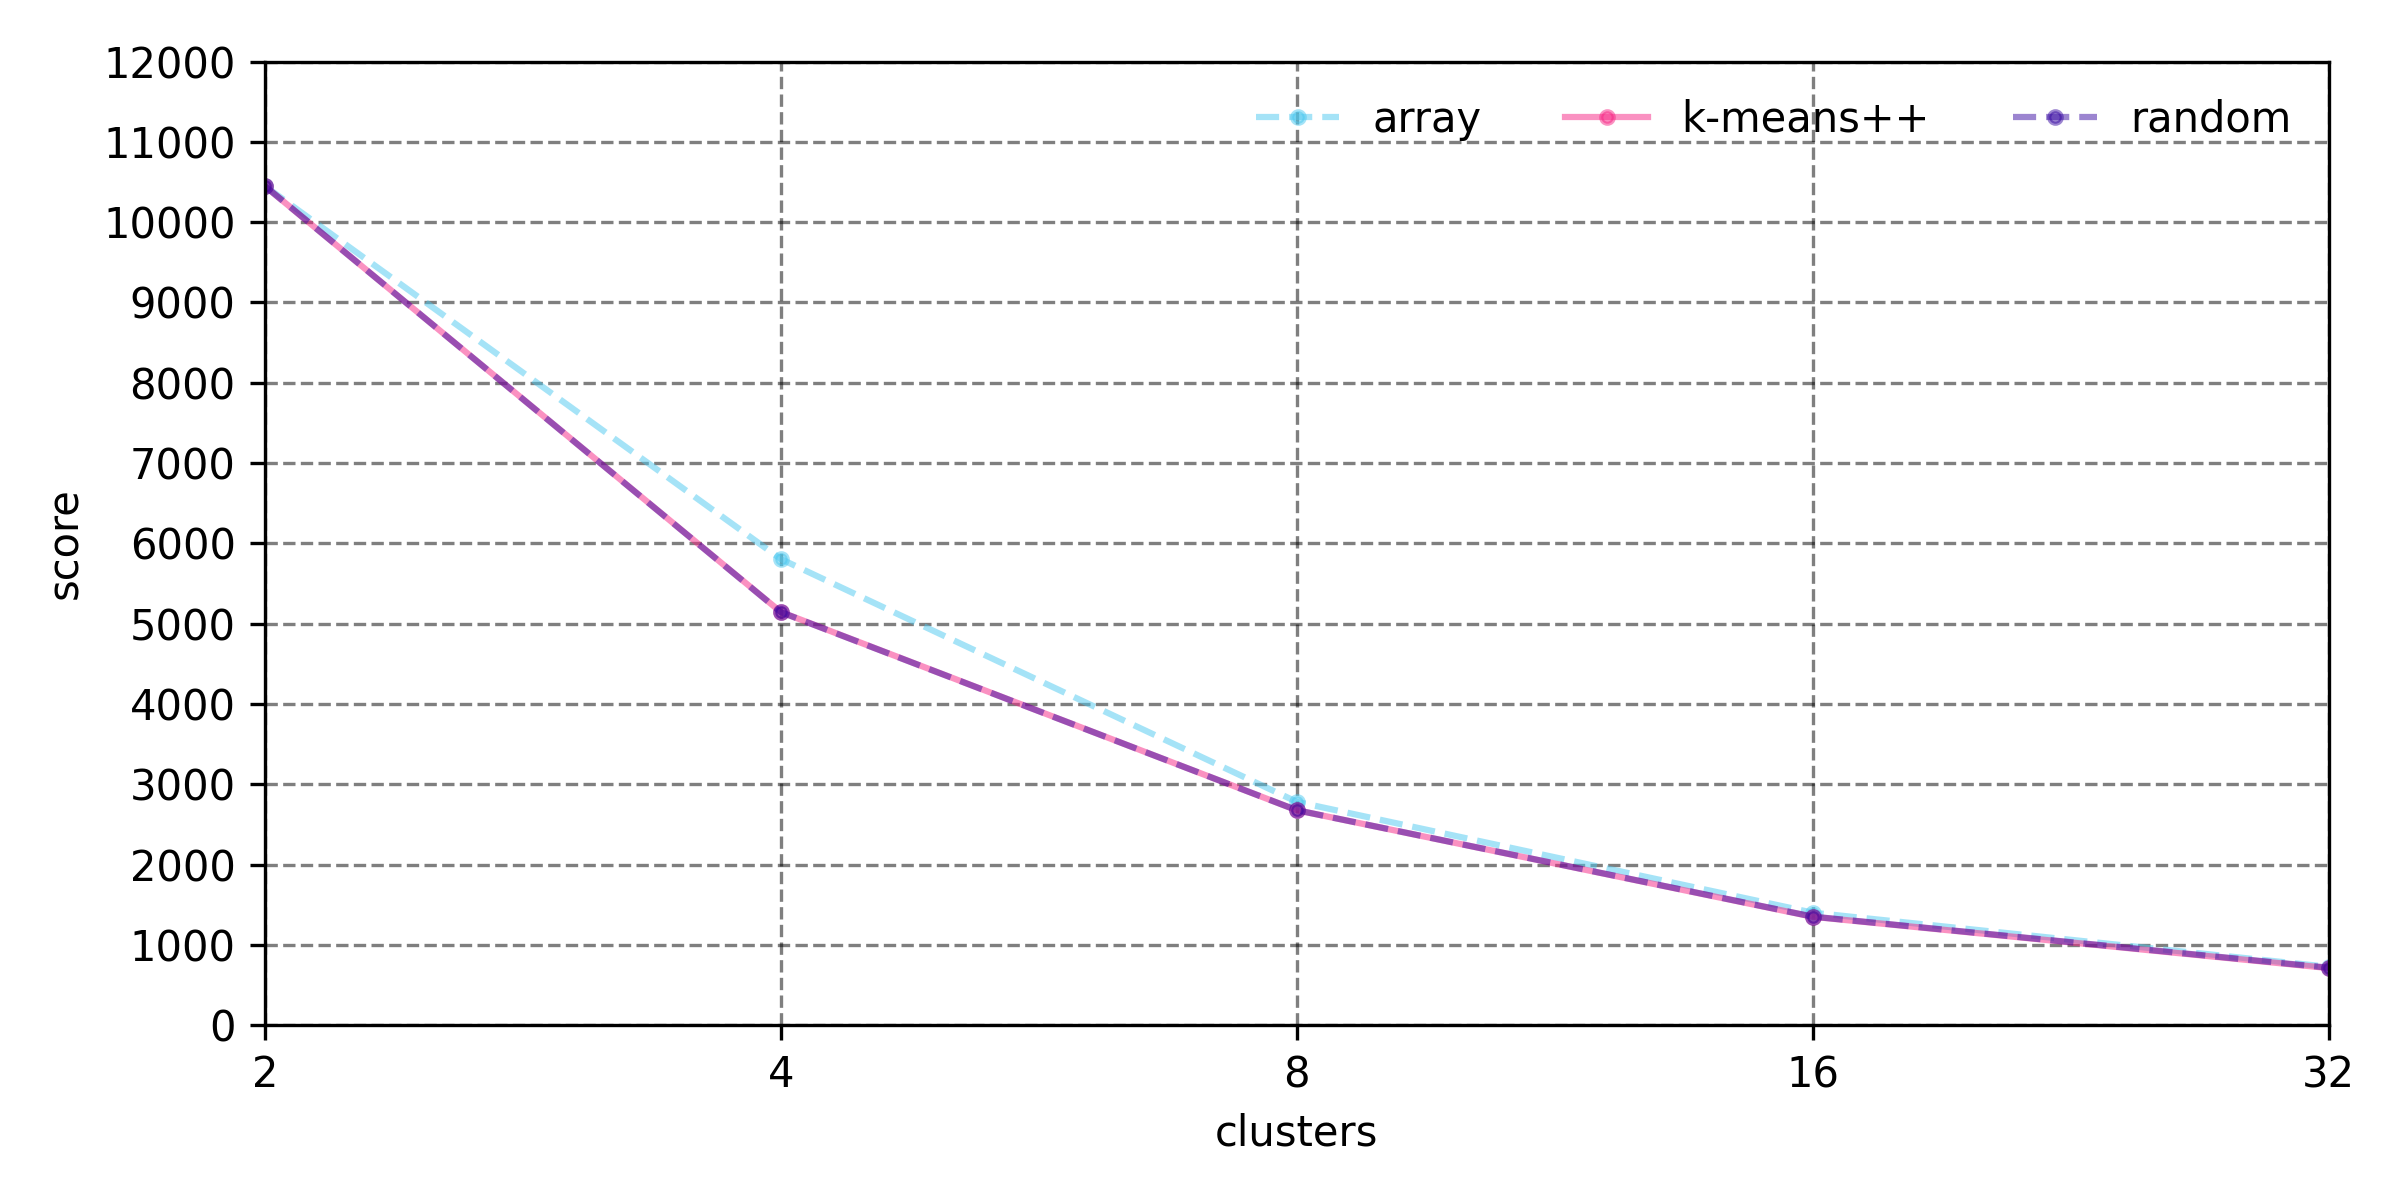
\includegraphics[width=16cm]{Graphics/Problema_04/mean_scores.png}
        \caption{Promedios de la función objetivo.}
    \end{subfigure}
    \begin{subfigure}{16cm}
        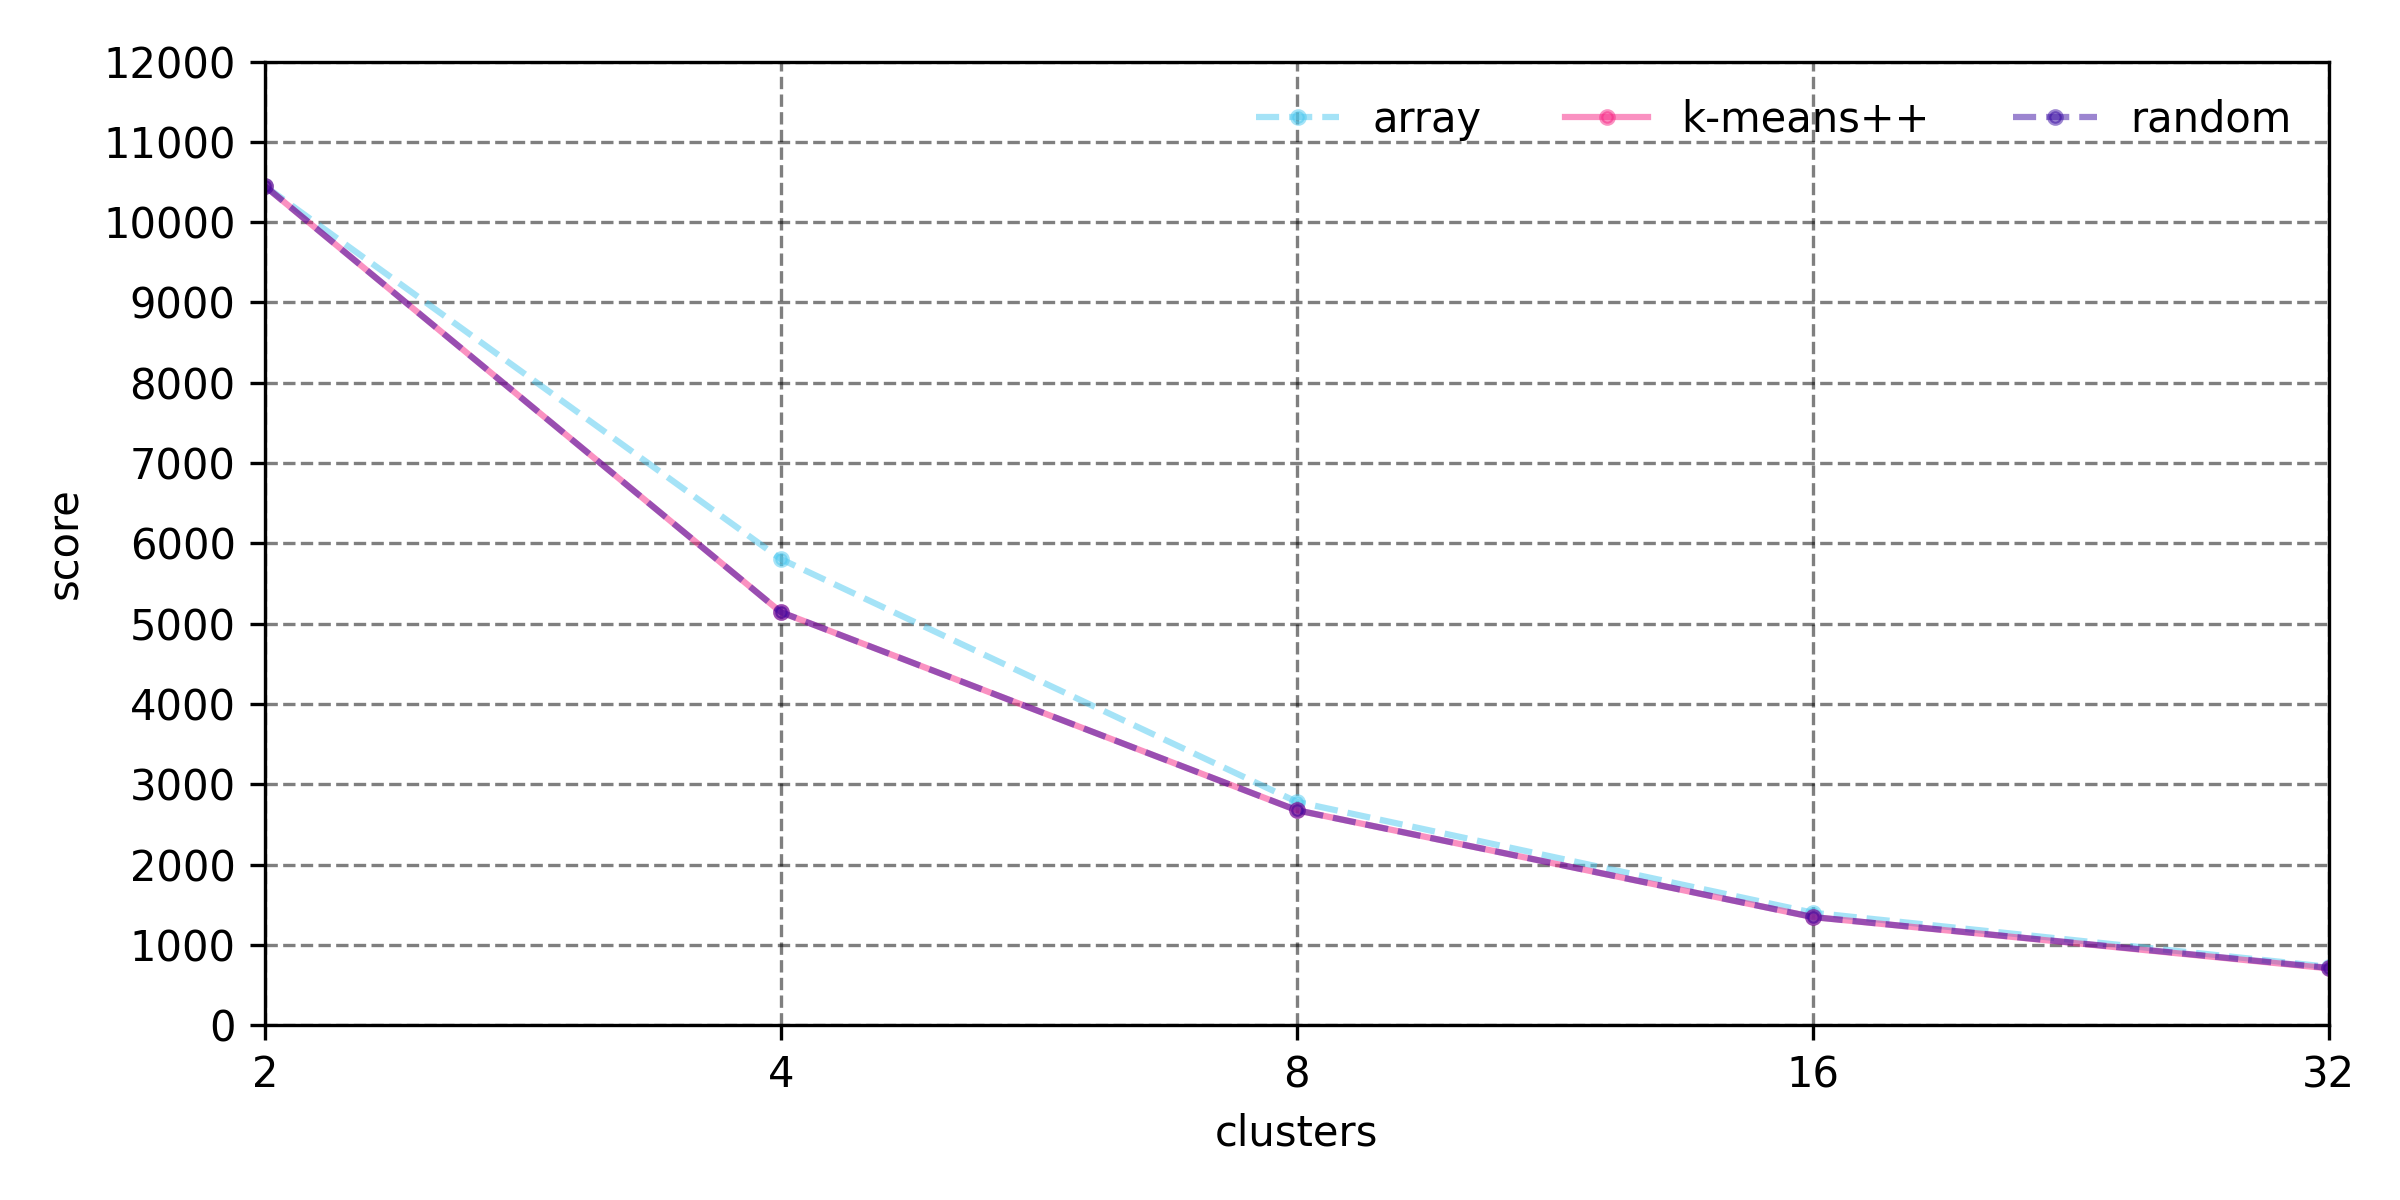
\includegraphics[width=16cm]{Graphics/Problema_04/minimum_scores.png}
        \caption{Mínimo de la función de objetivo.}
    \end{subfigure}
    \caption{Promedios y mínimo de la función objetivo de cada inicializador dado en el método de k-means.}
    \label{fig:problema_04_mean_and_minimum}
\end{figure}
\subsection*{Punto 02}

\textbf{Calcula y muestra el índice Fowlkes Mallows score (FM) usando el conjunto de entrenamiento. Muestra en una gráfica FM como una función de k, y comenta al respecto. Qué valor de k maximiza este criterio?}

En la figura \ref{fig:fowlkes_score} se visualiza el ínidice de Fowlkes Mallows para cada k calculada con el conjunto de entrenamiento. El índice de Fowlkes Mallows sigue una forma semejante a la figura \ref{fig:problema_05_minimum_score}. La diferencia se encuentra en el orden de magnitud de los valores de cada score obtenido. Si se quisiera máximizar el índice de Fowlkes Mallows se usaría k=2. Ya que para este valor se obtiene el valor máximo del índice.

\begin{figure}[H]
    \centering
    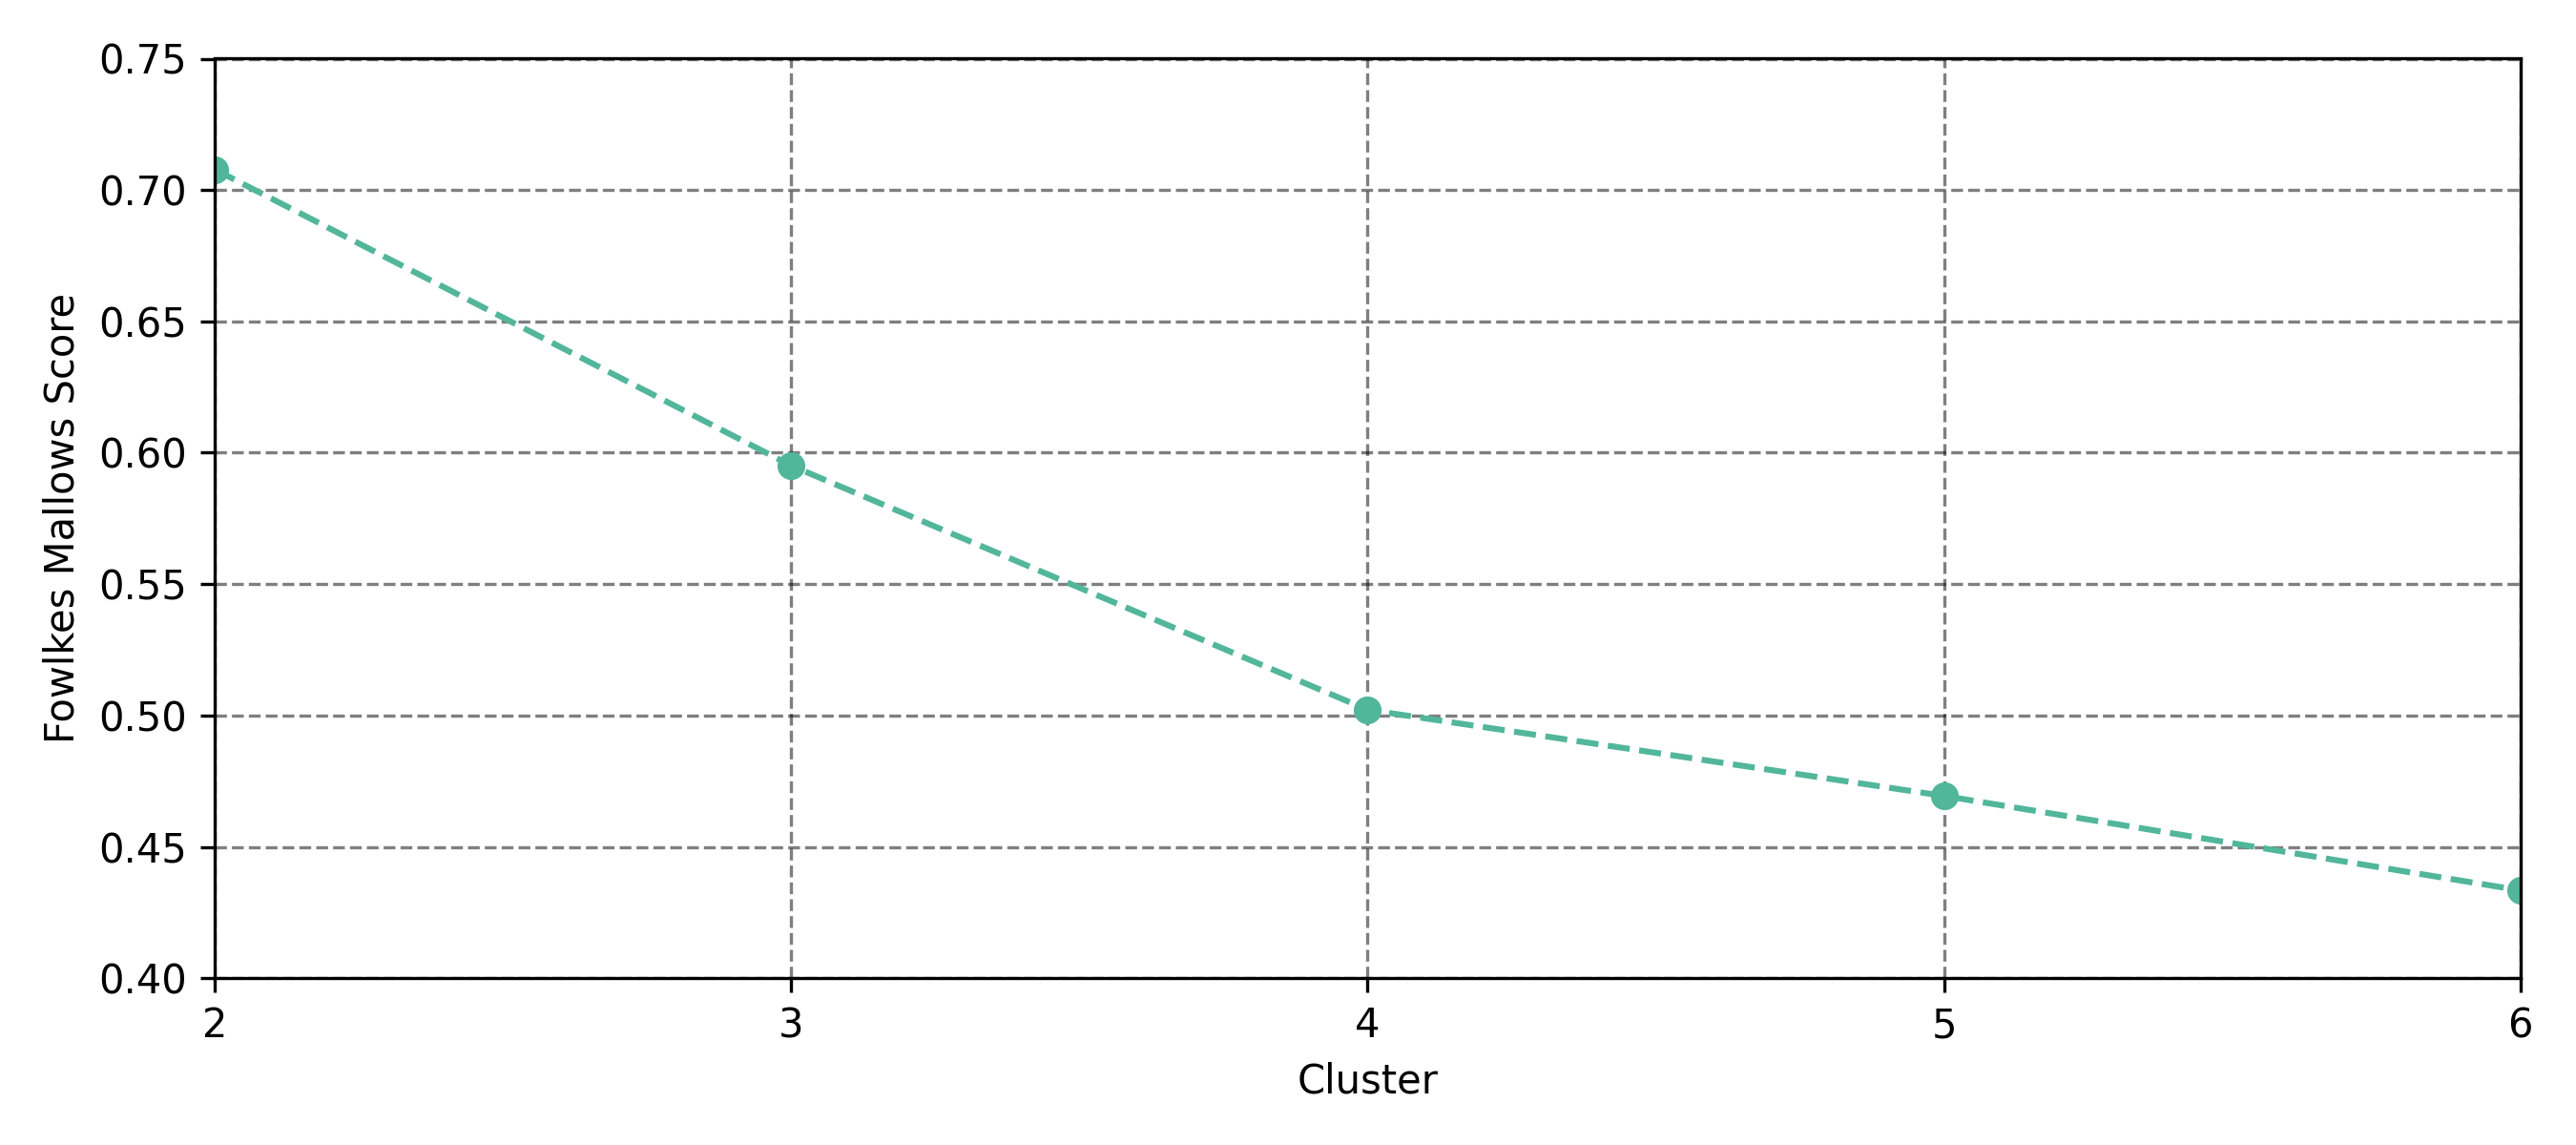
\includegraphics[width=15cm]{Graphics/Problema_05/fowlkes_mallows_score.png}
    \caption{Índice de Fowlkes Mallows obtenido a partir de los resultados usando el conjunto de entrenamiento del dataset \file{creditcard.csv}.}
    \label{fig:fowlkes_score}
\end{figure}